%\usepackage{xr}

% \externaldocument{note01}
% \externaldocument{note02}
% \externaldocument{note03}
% \externaldocument{note04}
% \externaldocument{note05}
% \externaldocument{note06}
% \externaldocument{note07}
% \externaldocument{note08}
% \externaldocument{note09}
% \externaldocument{note10}
% \externaldocument{note11}

\graphicspath{{./input/graphs/note05/}}


% \zexternaldocument{note01}
% \zexternaldocument{note02}
% \zexternaldocument{note03}
% \zexternaldocument{note04}
% \zexternaldocument{note05}
% \zexternaldocument{note06}
% \zexternaldocument{note07}
% \zexternaldocument{note08}
% \zexternaldocument{note09}
% \zexternaldocument{note10}
% \zexternaldocument{note11}
% \externaldocument{note12}



\week{5}
% \section*{Week 5. Lecture 13.}
\lecture{13}{Sequences in $\mathbb{C}$}
We introduce complex sequences and series, discuss their convergence and use them to construct complex power series. Then, we make several concrete connections with complex differentiable functions.

\section{Complex sequences.}

\subsection{Sequence limits}

\begin{definition}\label{definition:10.1} A sequence $\{z_n\}_{n=0}^{\infty}, z_n \in \mathbb{C}$, has limit $z$ (as $n \to \infty$) if for every $\epsilon > 0$ there exists $N = N(\epsilon) \in \mathbb{N}$ such that for all $n > N$, $|z_n - z| < \epsilon$. Notation: $\lim_{n \to \infty} z_n = z$.
\end{definition}
If the limit does not exist (or $\infty$), we say that the sequence diverges.

In other words, a sequence of complex numbers $\{z_n\}$ converges to the complex number $z$ iff at every neighborhood of $z$ there are almost all but finite number of points from the sequence: $\lim_{n \to \infty} z_n = z \iff \forall \epsilon > 0 \quad \exists N(\epsilon) \in \mathbb{N} \text{ s.t. for every } n > N(\epsilon) \quad |z_n - z| < \epsilon$.

\begin{claim}
If $\lim_{n \to \infty} z_n$ exists, then it is unique.
\begin{proof}
Assume $\lim_{n \to \infty} z_n = \tilde{z_1}$ and $\lim_{n \to \infty} z_n = \tilde{z_2}$. Then, for any $\epsilon > 0$ there exists $N_1 \in \mathbb{N}$ s.t. 
for every $n > N_1$, $|z_n - \tilde{z_1}| < \epsilon/2$. Also there exists $N_2 \in \mathbb{N}$ s.t. for every $n > N_2$, $|z_n - \tilde{z_2}| < \epsilon/2$. 
Choose $N = \max\{N_1, N_2\}$, then for every $n > N$, $|z_n - \tilde{z_1}| < \epsilon/2$ and $|z_n - \tilde{z_2}| < \epsilon/2$.

Thus $|\tilde{z_1} - \tilde{z_2}| = |\tilde{z_1} - z_n + z_n - \tilde{z_2}| \leq |\tilde{z_1} - z_n| + |z_n - \tilde{z_2}| < \epsilon/2 + \epsilon/2 = \epsilon$. Since this is true for any $\epsilon > 0$ we conclude that $\tilde{z_1} = \tilde{z_2}$.
\end{proof}
\end{claim}
Also, it is possible to show that the complex sequence $\{z_n\}$ converges to $z \iff$ the real sequence $\{|z_n - z|\}_{n=0}^{\infty}$ converges to 0 (\verifythis)

\begin{example}\label{example:12.1} Let $z_n = (\frac{i}{2})^n, n \in \mathbb{N}$. Then: $z_0 = 1, z_1 = \frac{i}{2}, z_2 = \frac{i^2}{4} = -\frac{1}{4}, z_3 = \frac{i^3}{8} = -\frac{i}{8}, z_4 = \frac{i^4}{16} = \frac{1}{16}, \dots$
\end{example}
This sequence converges to 0: $\lim_{n \to \infty} z_n = 0$. Can be demonstrated by proving that $|z_n|$ decreases to 0 as $n$ tends to infinity. (\checkthis{} By graphing the points $z_n$ check that the sequence
$\{z_n\}$ "spirals" in toward the origin $(0)$ in the $z$-plane.

\begin{example}\label{example:12.2} Let $z_n = (2i)^n: z_0 = 1, z_1 = 2i, z_2 = -4, z_3 = -8i, \dots$. This sequence diverges: one can show that $\{|z_n|\}_{n=0}^{\infty}$ is unbounded increasing sequence \{namely, $|z_n|$ gets arbitrarily large\}.
\end{example}

\begin{example}\label{example:12.3} Let $z_n = (i)^n: z_0 = 1, z_1 = i, z_2 = -1, z_3 = -i, z_4 = 1, z_5 = i, \dots$. This is a bounded sequence ($|z_n| \leq 1$ for any $n$), but $\lim_{n \to \infty} z_n$ does not exist: there is no $z$ such that almost all but finitely many points of the sequence are in a small neighborhood of some $z$: 
    
    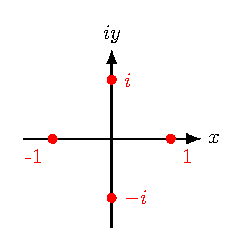
\includegraphics{img_graph1.pdf}
    
    $z_n$ jumps at every step.
\end{example}

Important real sequence (limit): let $a_n = (1 + \frac{a}{n})^n$ for some $a$. Then $\lim_{n \to \infty} a_n = (1 + \frac{a}{n})^n = e^a$.

\begin{example}\label{example:12.4} $\lim_{n \to \infty} (1 + \frac{i}{n})^n = e^i, \quad \lim_{n \to \infty} (1 - \frac{i}{n})^n = \lim_{n \to \infty} (1 + \frac{-i}{n})^n = e^{-i} = \frac{1}{e^i}$.
\end{example}

\begin{proposition} \zlabel{proposition:10.1} 
    If the sequences $\{z_n\}, \{w_n\}$ of complex numbers converge, then so the sequences $\{z_n \pm w_n\}, \{z_n \cdot w_n\}$, 
    and if $w_n \neq 0$ also $\{\frac{z_n}{w_n}\}$, and 
    \[\lim_{n \to \infty} (z_n \pm w_n) = \lim_{n \to \infty} z_n \pm \lim_{n \to \infty} w_n; \quad \lim_{n \to \infty} z_n w_n = \lim_{n \to \infty} z_n \lim_{n \to \infty} w_n.\]

If $\lim_{n \to \infty} w_n \neq 0$, then: $\lim_{n \to \infty} \frac{z_n}{w_n} = \frac{\lim_{n \to \infty} z_n}{\lim_{n \to \infty} w_n}$.
\end{proposition}

\section{Complex (scalar) series.}

\subsection{Series convergence}

\begin{definition}\label{definition:11.1} 
    The complex (scalar) series $\sum_{n=1}^{\infty} z_n$ converges to the value $s \in \mathbb{C}$ if the sequence of partial sums $\{S_N\}_{N=0}^{\infty}, S_N = z_0 + z_1 + \dots + z_N$ converges to $s$. 
    The value $s$ is called the sum of the series. If the limit does not exist (or $\infty$) ($\lim_{N \to \infty} S_N$) then the series diverges. If the series converges to some value $s$, then $s$ is unique.
\end{definition}

\begin{remark}
Furthermore: if $r_N = S - S_N = \sum_{n=N+1}^{\infty} z_n$, then it is possible to show that $\sum_{n=0}^{\infty} z_n = S \iff \lim_{N \to \infty} r_N = 0$. 
Namely, the \emphi{tail} of the series converges to 0.
\end{remark}
From Def (\ref{definition:11.1}) we immediately conclude:
\begin{proposition}\label{proposition:11.1} If $\sum_{n=0}^{\infty} z_n$ converges, then $\lim_{n \to \infty} z_n = 0$.
\begin{proof}
    By Def (\ref{definition:11.1}): If $\sum_{n=0}^{\infty} z_n = S$, then $\lim_{N \to \infty} S_N = \lim_{N \to \infty} \sum_{n=0}^{N} z_n = S$. On the other hand: $S_N - S_{N-1} = (z_0 + z_1 + \dots + z_N) - (z_0 + z_1 + \dots + z_{N-1}) = z_N$
    $\implies \lim_{N \to \infty} z_N = \lim_{N \to \infty} (S_N - S_{N-1}) = \lim_{N \to \infty} S_N - \lim_{N \to \infty} S_{N-1} = S - S = 0$ by Prop 10.1(\zref{proposition:10.1}). $s$ is unique.
\end{proof}
\end{proposition}
The contrapositive statement is often called the Test for Divergence.

\begin{proposition}[Test for Divergence]\label{proposition:11.2} (Test for Divergence) Let $\{z_n\}_{n=0}^{\infty} \in \mathbb{C}$. If $\lim_{n \to \infty} z_n \neq 0$ (or does not exist), then the series $\sum_{n=0}^{\infty} z_n$ diverges.
\end{proposition}

\begin{remark}
The converse of Prop 11.2(\ref{proposition:11.2}) is false: $\lim_{n \to \infty} \frac{1}{n} = 0$, but the series $\sum_{n=1}^{\infty} \frac{1}{n}$ diverges!
\end{remark}
As expected there is an immediate relation between convergence or divergence of complex sequences and series to that of real ones.

\begin{proposition}\label{proposition:11.3} Let $\{z_n\}_{n=0}^{\infty}, z_n$ be the complex sequence and the complex series. Suppose that $z = x + iy$ and $S = u + iv$. Then:
\begin{enumerate}
    \item $\lim_{n \to \infty} z_n = z \iff \lim_{n \to \infty} x_n = x$ and $\lim_{n \to \infty} y_n = y$ (for $z_n = x_n + iy_n$)
    \item $\sum_{n=0}^{\infty} z_n = S \iff \sum_{n=0}^{\infty} x_n = u$ and $\sum_{n=0}^{\infty} y_n = v$
\end{enumerate}
\begin{proof}
    \begin{enumerate}
        \item follows directly from Def 10.1(\ref{definition:10.1}) and the application of triangle inequality: $|x_n - x|, |y_n - y| \leq |z_n - z| \leq |x_n - x| + |y_n - y|$
        \item is proved by decomposing the complex sum into real and imaginary parts $\sum_{n=0}^{\infty} z_n = \sum_{n=0}^{\infty} x_n + i\sum_{n=0}^{\infty} y_n$ and a careful use of 1) [FINISH!]
    \end{enumerate}
\end{proof}
\end{proposition}

Hint: If $\sum_{n=0}^{\infty} x_n = u, \sum_{n=0}^{\infty} y_n = v \implies$ obvious. Assume $\sum_{n=0}^{\infty} z_n = S$, define $X_N = \sum_{n=0}^{N} x_n, Y_N = \sum_{n=0}^{N} y_n$, apply 1) to $S_N = \sum_{n=0}^{N} z_n$.

In much of what follows, we can use Prop 11.3 and results in real sequences and series - these are left as an exercise. For example, Prop 10.1 and an analogous proposition for the series:

\begin{proposition} \label{proposition:11.4} Suppose that $\sum_{n=0}^{\infty} z_n = S, \sum_{n=0}^{\infty} w_n = t$ are two convergent series. Let $\alpha \in \mathbb{C}$. Then,
\begin{enumerate}
    \item $\sum_{n=0}^{\infty} (z_n \pm w_n) = S \pm t$ (converges to $S \pm t$)
    
    \item $\sum_{n=0}^{\infty} \alpha z_n = \alpha S$ (converges to $\alpha S$)
\end{enumerate}

\begin{proof} (EXERCISE - exactly as in the real case - partial sums).
\end{proof}
\end{proposition}

\begin{example} \label{example:13.1} (Key example - Geometric series)

Suppose that $|z| < 1$. We claim that the series $\sum_{n=0}^{\infty} z^n$, called the Geometric series, converges.
\begin{claim}\label{claim:11.5}
    $\sum_{n=0}^{\infty} z^n$ converges (if $|z| < 1$) and $\sum_{n=0}^{\infty} z^n = \frac{1}{1-z}$.
\end{claim}
\begin{proof}
    We prove it using Def 11.1: we will show that the sequence of partial sums converges to $\frac{1}{1-z}$.
    Need to show: $\lim_{N \to \infty} S_N = \lim_{N \to \infty} \sum_{n=0}^{N} z^n = \frac{1}{1-z}$.
    
    First, we obtain a closed formula for $S_N$ as follows.
    \begin{align*}
        S_N &= 1 + z + z^2 + \dots + z^N \\
        z \cdot S_N &= z + z^2 + z^3 + \dots + z^{N+1} \\
        &\implies S_N - zS_N = S_N(1-z) = 1 - z^{N+1} \\
        &\implies S_N = \frac{1 - z^{N+1}}{1-z}
    \end{align*}
\end{proof}
Now we use this formula to compute the limit
\[ \left| \frac{1}{1-z} - S_N \right| = \left| \frac{1}{1-z} - \frac{1 - z^{N+1}}{1-z} \right| = \left| \frac{z^{N+1}}{1-z} \right| = \frac{|z|^{N+1}}{|1-z|} \]
Since $|z| < 1 \implies \lim_{N \to \infty} |z|^N = 0$ (from what we know about real sequences). Therefore $\left| \frac{1}{1-z} - S_N \right| \xrightarrow{N \to \infty} 0 \implies \lim_{N \to \infty} S_N = \frac{1}{1-z}$.
\end{example}

% \section*{Lectures 14+15.}
\lecture{14+15}{Absolute convergence?! WTH is that?}

Now we introduce the notion of absolute convergence.

\begin{definition}\label{definition:11.2} The series $\sum_{n=0}^{\infty} z_n$ converges absolutely if the series of the moduli of the terms $\sum_{n=0}^{\infty} |z_n|$ converges.
\end{definition}

\begin{remark}
Note: (The Geometric series) For $|z| < 1$, $\sum_{n=0}^{\infty} |z|^n$ converges. Namely, the geometric series converges absolutely.
\begin{proof}
    Follow exactly the same steps as in Ex 13.1, replace $z$ by $|z|$.
\end{proof}
\end{remark}

The definition of absolute convergence is subtle: Series can converge, but not absolutely: $\sum_{n=1}^{\infty} \frac{(-1)^n}{n}$ converges, but $\sum_{n=1}^{\infty} |\frac{(-1)^n}{n}| = \sum_{n=1}^{\infty} \frac{1}{n}$ diverges.

The absolute convergence *however* always implies convergence:

\begin{proposition}\label{proposition:11.6} If $\sum_{n=0}^{\infty} |z_n|$ converges, then $\sum_{n=0}^{\infty} z_n$ converges.
\begin{proof}
    We have $|z_n| = \sqrt{x_n^2 + y_n^2} \geq |x_n|, |y_n|$, therefore using the Comparison test for positive (real) series we get that $\sum_{n=0}^{\infty} |x_n|$ 
    and $\sum_{n=0}^{\infty} |y_n|$ converge $\implies$ (by analogous statement for real series) $\sum_{n=0}^{\infty} x_n$ and $\sum_{n=0}^{\infty} y_n$ converge. 
    Thus, by Prop 11.3(\ref{proposition:11.3}) 2) $\sum_{n=0}^{\infty} z_n$ converges.
\end{proof}
\end{proposition}

Now we state 3 very useful tests for convergence of complex series.

\begin{proposition} \label{proposition:11.7} Let $\sum_{n=0}^{\infty} a_n, a_n \in \mathbb{C}$ be a complex series.

\begin{enumerate}
    \item \textbf{Ratio-Test:} Consider the limit $\lim_{n \to \infty} \left| \frac{a_{n+1}}{a_n} \right| = \lim_{n \to \infty} \frac{|a_{n+1}|}{|a_n|} = L$
    \begin{itemize}
        \item If the limit exists and $L < 1$, then the series $\sum_{n=0}^{\infty} a_n$ converges absolutely.
        \item If the limit exists and $L > 1$, then the series $\sum_{n=0}^{\infty} a_n$ diverges.
        \item If $L = 1$ or the limit does not exist, then the test is inconclusive \{namely, there are examples of convergent and divergent series\}.
    \end{itemize}
    \item \textbf{Root (Cauchy) Test:} Consider the limit $\lim_{n \to \infty} \sqrt[n]{|a_n|} = L$
    \begin{itemize}
        \item If the limit exists and $L < 1$, then the series $\sum_{n=0}^{\infty} a_n$ converges absolutely.
        \item If the limit exists and $L > 1$, then the series $\sum_{n=0}^{\infty} a_n$ diverges.
        \item If $L = 1$ or does not exist, then the test is inconclusive.
    \end{itemize}
    \item \textbf{Comparison Test:}
    \begin{itemize}
        \item If $0 \leq |a_n| < r_n$ and the positive real series $\sum_{n=0}^{\infty} r_n$ converges, then $\sum_{n=0}^{\infty} a_n$ converges absolutely.
        \item If $|a_n| > r_n \geq 0$ and $\sum_{n=0}^{\infty} r_n$ diverges, then $\sum_{n=0}^{\infty} a_n$ diverges.
    \end{itemize}

\end{enumerate}
\end{proposition}
\begin{proof}
    Ratio Test: If $L > 1$, then the sequence $\{|a_n|\}$ is increasing (for sufficiently large $n$), therefore the series diverges by the Test for Divergence.
    
    Suppose that $L < 1$. Choose a number $r$ such that $L < r < 1$. Since $\lim_{n \to \infty} \left| \frac{a_{n+1}}{a_n} \right| = L$ there exists $N \in \mathbb{N}$ such that for all $n \geq N: \left| \frac{|a_{n+1}|}{|a_n|} - L \right| < \epsilon$. Set $\epsilon = a_N$. Then we have $|a_{N+1}| \leq r|a_N| = |a|r$, $|a_{N+2}| \leq r|a_{N+1}| < |a|r^2$ and, in general $|a_{N+k}| \leq |a|r^k$. Therefore for $n \geq N$ the terms of the series $\sum_{n=0}^{\infty} |a_n|$ are bounded by the terms of a convergent geometric series (since $0 \leq r < 1$), therefore $\sum_{n=0}^{\infty} |a_n|$ converges by the Comparison Test (for real series), namely, $\sum_{n=0}^{\infty} a_n$ converges absolutely.
    
    Root Test and Comparison Test: EXERCISE!
\end{proof}

\begin{example}\label{example:13.2} Check the convergence of the following series:
    \begin{enumerate}
        \item  $\sum_{n=0}^{\infty} (2i)^n$ 
        \item  $\sum_{n=0}^{\infty} \left(\frac{1+i}{2}\right)^n$ 
        \item  $\sum_{n=0}^{\infty} \frac{(4i)^n}{n!}$
    \end{enumerate}
\begin{soln}
    \begin{enumerate}
        \item We use Comparison Test as follows: $a_n = (2i)^n \implies |a_n| = (|2i|)^n = |2|^n = 2^n > (\frac{3}{2})^n$. Since $\sum_{n=0}^{\infty} (\frac{3}{2})^n$ diverges (for example, by the Test for Divergence, since $\lim_{n \to \infty} (\frac{3}{2})^n = \infty \neq 0$) by Comparison Test $\sum_{n=0}^{\infty} (2i)^n$ diverges.
    
        \item Let us apply the Root Test: $a_n = \left(\frac{1+i}{2}\right)^n$
    $\implies \lim_{n \to \infty} \sqrt[n]{|a_n|} = \lim_{n \to \infty} \sqrt[n]{\left|\frac{1+i}{2}\right|^n} = \lim_{n \to \infty} \frac{|1+i|}{2} = \frac{\sqrt{2}}{2} = \frac{1}{\sqrt{2}} < 1$
    $\implies \sum_{n=0}^{\infty} \left(\frac{1+i}{2}\right)^n$ converges absolutely.
    
    \item Let us apply the Ratio Test: $a_n = \frac{(4i)^n}{n!}$
    
    \begin{align*}
         \implies \lim_{n \to \infty} \left| \frac{a_{n+1}}{a_n} \right| = \lim_{n \to \infty} \left| \frac{\frac{(4i)^{n+1}}{(n+1)!}}{\frac{(4i)^n}{n!}} \right| &= \lim_{n \to \infty} \left| \frac{(4i)^{n+1}}{(n+1)!} \cdot \frac{n!}{(4i)^n} \right| \\
         & = \lim_{n \to \infty} \frac{|4i|}{n+1} = \lim_{n \to \infty} \frac{4}{n+1} = 0 < 1 
    \end{align*}
    
    $\implies $ converges absolutely.
    \end{enumerate}
\end{soln}
\end{example}

\section{Complex Power Series}

\subsection{Power series basics}
\begin{definition}\label{definition:12.1} 
    The series $\sum_{n=0}^{\infty} a_n(z-z_0)^n, a_n \in \mathbb{C}, n \in \mathbb{N}$, is called a power series centered at $z = z_0$ (about $z = z_0$).
\end{definition}

A power series is an example of complex series where the sequence $z_n$ from Def 11.1(\ref{definition:11.1}) is of the special form $\{a_n(z-z_0)^n\}$ - involves variable $z$. 
Thus, the convergence or divergence of a power series may depend on the values of the variable $z$. If $z_0 = 0$, the power series are of the form $\sum_{n=0}^{\infty} a_n z^n$.

\begin{remark}
From Def 12.1(\ref{definition:12.1}) every power series $\sum_{n=0}^{\infty} a_n(z-z_0)^n$ converges for at least one point $z = z_0$.
\end{remark}
Next theorem tells us that convergence at one point guarantees convergence on some small disc around $z_0$. We prove it for the case $z_0 = 0$ (for simplicity of notation), the general case $z_0 \neq 0$ is proved in exactly the same way.

\begin{theorem}[Abel]\label{theorem:12.1}
    If $\sum_{n=0}^{\infty} a_n z^n$ converges at $z_0 \neq 0$, then it converges absolutely for any $z$ with $|z| < |z_0|$.
    Namely, if the series converges at a point $z_0$, then it converges absolutely at every interior point of the disc centered at 0 of radius $|z_0|$.
\end{theorem}
    \begin{proof}
        Since $\sum_{n=0}^{\infty} a_n z_0^n$ converges by (Prop 11.1(\ref{proposition:11.1})) $\lim_{n \to \infty} a_n z_0^n = 0$, 
        thus $\{a_n z_0^n\}$ is a bounded sequence: there exists $M \in \mathbb{N}$ such that for every $n \in \mathbb{N}$ $|a_n z_0^n| < M$.
        Write the modulus of the general term of the series as: $|a_n z^n| = |a_n z_0^n \cdot \frac{z^n}{z_0^n}| = |a_n z_0^n| \left| \frac{z}{z_0} \right|^n < M \left| \frac{z}{z_0} \right|^n$
        $\implies$ since $|z| < |z_0|$, namely $\left| \frac{z}{z_0} \right| < 1$, the general term of the positive series $\sum_{n=0}^{\infty} |a_n z^n|$ is smaller than the one of the positive geometric 
        series $\sum_{n=0}^{\infty} M \left| \frac{z}{z_0} \right|^n \implies$ by Comparison Test
        ( $\sum_{n=0}^{\infty} |a_n z^n|$ ) converges $\implies \sum_{n=0}^{\infty} a_n z^n$ converges absolutely.
    \end{proof}
    
\begin{corollary}\label{corollary:12.1}
    If $\sum_{n=0}^{\infty} a_n z^n$ converges at $z = z_1$, then it diverges for every $z$ with $|z| > |z_1|$.
\end{corollary}

\begin{definition}\label{definition:12,2} If the series $\sum_{n=0}^{\infty} a_n z^n$ converges for all $z \in U \subseteq \mathbb{C}$, then its sum defines a function on $U$.
\end{definition}

\begin{example}[ \ref{example:13.1}(continued)] \label{example:13.1continued} $\sum_{n=0}^{\infty} z^n$ - power series centered at $z_0 = 0$, $a_n = 1$ for all $n$. Converges on the open unit disc $U = \{z \in \mathbb{C}: |z| < 1\}$ (converges absolutely!), and equal to the function $f(z) = \frac{1}{1-z}$ on $U$.
\end{example}

Next proposition tells us where the power series converges. The proof is omitted.

\begin{proposition}\label{proposition:12.1} Given a power series $\sum_{n=0}^{\infty} a_n (z - z_0)^n$ there exists $0 \leq R \leq \infty$ \{a real non-negative number or else infinity\} such that if $|z - z_0| < R$, then $\sum_{n=0}^{\infty} a_n (z - z_0)^n$ converges absolutely and if $|z - z_0| > R$, then $\sum_{n=0}^{\infty} a_n (z - z_0)^n$ diverges.
\end{proposition}

The value $R$ is called the radius of convergence of power series.

A very useful formulae for computing the radius of convergence of power series:

\begin{itemize}
    \item $R = \lim_{n \to \infty} \left| \frac{a_n}{a_{n+1}} \right|$ \{for $\sum_{n=0}^{\infty} a_n (z - z_0)^n$\}
    \item Cauchy-Hadamard formula: $R = \lim_{n \to \infty} \frac{1}{\sqrt[n]{|a_n|}}$
\end{itemize}

\begin{example}\label{example:14.1} Find the radius of convergence of $\sum_{n=0}^{\infty} (n+i)z^n$.
\begin{soln}
     $a_n = n + i \implies |a_n| = \sqrt{n^2 + 1}$.

    Using Cauchy-Hadamard formula and that $\lim_{n \to \infty} \sqrt[n]{n} = 1$ we get: 
    \[ R = \lim_{n \to \infty} \frac{1}{\sqrt[n]{\sqrt{n^2 + 1}}} = 1.\] 
    Namely, the series converges absolutely for $|z| < 1$.
\end{soln}
\end{example}

\begin{remark}
    The power series with the radius of convergence $R$ on the circle $|z - z_0| = R$ (or $|z| = R$ if $z_0 = 0$) may converge or diverge or converge at some points and diverge at others.
\end{remark}

\begin{example}\label{example:14.2} 
    \begin{enumerate}
        \item The geometric series $\sum_{n=0}^{\infty} z^n$ - the radius of convergence $R = 1$ and the series diverges at any point on the circle $|z| = 1$ (by the Test for Divergence).
        \item $\sum_{n=0}^{\infty} \frac{z^n}{n^2}$: The radius of convergence $R = 1$ [\verifythis]
        
        and the series converges (absolutely) for any $|z| \leq 1$.
        \item One can prove: the series $1 + z + \frac{z^2}{2} + \frac{z^3}{3} + \dots + \frac{z^n}{n} + \dots$ with the radius of convergence $R = 1$, diverges at $z = 1$ and converges at 
        all other points $|z| = 1$ (not absolutely!).
    \end{enumerate}
\end{example}

\begin{definition}\label{definition:12.3} The disc of convergence of the power series $\sum_{n=0}^{\infty} a_n (z - z_0)^n$ is given by $D = \{z \in \mathbb{C}: |z - z_0| < R\}$ and we 
    write $f(z)$ for the sum of the series on this disc.
\end{definition}

\begin{proposition} \label{proposition:12.2} Suppose the power series $\sum_{n=0}^{\infty} a_n (z - z_0)^n$ has disc of convergence $D$. Then,
    \begin{enumerate}
        \item $f(z) = \sum_{n=0}^{\infty} a_n (z - z_0)^n$ is analytic on $D$ \{differentiable at every $z \in D$\}
        \item For all $z \in D$ the series $\sum_{n=0}^{\infty} na_n (z - z_0)^{n-1}$ is absolutely convergent and has sum $f'(z)$ (the derivative of $f$ at $z$).
    \end{enumerate}
\end{proposition}

Note: From Prop 12.2(\ref{proposition:12.2}): $f(z) = \sum_{n=0}^{\infty} a_n (z - z_0)^n$ is differentiable arbitrarily many times at any $z$ in the disc of convergence 
of the series (namely, we can define its higher derivatives).

\begin{definition} \label{definition:12.4} For any $z \in \mathbb{C}$ we define the exponential function as the sum of the following series
\[ e^z = 1 + z + \frac{z^2}{2!} + \frac{z^3}{3!} + \dots = \sum_{n=0}^{\infty} \frac{z^n}{n!} \]
If $z$ is real, we get the usual expansion of $e^x$ to series.
\end{definition}

\begin{claim}
Claim: $e^z$ is well-defined for all $z \in \mathbb{C}$, namely $R = \infty$.

\begin{proof}
By Ratio Test:
\[ \lim_{n \to \infty} \left| \frac{a_{n+1}}{a_n} \right| = \lim_{n \to \infty} \left| \frac{\frac{z^{n+1}}{(n+1)!}}{\frac{z^n}{n!}} \right| = \lim_{n \to \infty} \left| \frac{z}{n+1} \right| = 0 < 1 \quad \text{for all } z \in \mathbb{C} \]
$\implies \sum_{n=0}^{\infty} \frac{z^n}{n!}$ converges absolutely for all $z \in \mathbb{C}$.
\end{proof}
\end{claim}
\begin{proposition}\label{proposition:12.3} $e^z$ is entire and $(e^z)' = e^z$.
\begin{proof}
    By Prop 12.2(\ref{proposition:12.2}) 1) $e^z$ is analytic for every $z \in \mathbb{C} \implies$ entire (since $R = \infty$). By Prop 12.2 (\ref{proposition:12.2}) 2): $(e^z)' = \sum_{n=1}^{\infty} \frac{nz^{n-1}}{n!} = \sum_{n=1}^{\infty} \frac{z^{n-1}}{(n-1)!} = \sum_{n=0}^{\infty} \frac{z^n}{n!} = e^z$.
\end{proof}
\end{proposition}

\begin{proposition} \label{proposition:12.4} For any $z_1, z_2 \in \mathbb{C}: e^{z_1} \cdot e^{z_2} = e^{z_1 + z_2}$.
\begin{proof}
    
    By Def 12.4(\ref{definition:12.4}): $e^{z_1} = \sum_{n=0}^{\infty} \frac{z_1^n}{n!}, \quad e^{z_2} = \sum_{n=0}^{\infty} \frac{z_2^n}{n!}$.
    
    These are absolutely convergent series $\implies$ we can multiply them:
    $e^{z_1 + z_2} = 1 + (z_1 + z_2) + \frac{1}{2!}(z_1 + z_2)^2 + \dots + \frac{1}{n!}(z_1 + z_2)^n + \dots = 1 + (z_1 + z_2) + \left(\frac{z_1^2}{2!} + z_1z_2 + \frac{z_2^2}{2!}\right) + \dots + \left(\frac{z_1^n}{n!} + \frac{z_1^{n-1}}{(n-1)!}z_2 + \dots + \frac{z_2^n}{n!}\right) + \dots = e^{z_1}e^{z_2}$
\end{proof}
\end{proposition}

Now we can define trigonometric functions as power series:

\begin{definition}\label{definition:12.5} For any $z \in \mathbb{C}, |z| < \infty$
    \begin{align*} 
        & \sin z = \text{Im } e^{iz} = z - \frac{z^3}{3!} + \frac{z^5}{5!} - \dots = \sum_{n=0}^{\infty} \frac{(-1)^n}{(2n+1)!}z^{2n+1} \\
        & \cos z = \text{Re } e^{iz} = 1 - \frac{z^2}{2!} + \frac{z^4}{4!} - \dots = \sum_{n=0}^{\infty} \frac{(-1)^n}{(2n)!}z^{2n} 
    \end{align*}
For real $z$ this definition coincide with Taylor series expansion of $\sin x$ and $\cos x$ about $x = 0$.

\end{definition}
